\documentclass[12pt]{article}
\usepackage{graphicx}
\usepackage{fancyhdr}
\usepackage{setspace}
\usepackage[utf8]{inputenc}
\usepackage[T1]{fontenc}
\usepackage[a4paper,margin=1in]{geometry}   % 1 inch margins on all sides
\usepackage{mathptmx}                        % Times New Roman-equivalent font
\usepackage{titlesec}
\usepackage{natbib}
\usepackage[nottoc]{tocbibind}
\usepackage[hidelinks]{hyperref}
\usepackage{tikz}
\usepackage{amsmath}
\usepackage{amssymb}
\usepackage{indentfirst}
\usetikzlibrary{arrows.meta, positioning, calc}
\usepackage{float}
\usepackage{cleveref}
%INFO
\newcommand{\rptTitle}{Design and Motion Control of a Quadruped Robot on Gazebo}
\newcommand{\rptStudentName}{Arda Gencer}
\newcommand{\rptStudentID}{00034124}
\newcommand{\rptStartDate}{24.08.2026}
\newcommand{\rptEndDate}{20.09.2026}
\newcommand{\rptCompany}{BİTES Savunma, Havacılık ve Uzay Teknolojileri Yazılım Elektronik Ticaret A.\c{S}.}
\newcommand{\rptSupervisor}{Kadir G\"uney}
\newcommand{\rptSubmissionDate}{DD.09.2026}
\newcommand{\rptProgram}{Computer Science and Engineering / Mechatronics Engineering}
% Optional logo: put a file named sabanci_logo.png next to this .tex file.
% If it's not there, the title page just skips it -- no error either way.
\newcommand{\rptLogoFile}{sabanci_logo.png}
% ---- Paragraph style: double spacing, no extra space between paragraphs,
%      first line indented, body justified (LaTeX justifies by default) ----

\pagestyle{fancy}
\setlength{\headheight}{14pt}
\fancyhf{}
\renewcommand{\headrulewidth}{0pt}
\fancyhead[C]{\small Design and Motion Control of a Quadruped Robot on Gazebo}
\fancyfoot[C]{\thepage}
\begin{document}
\begin{titlepage}
\centering
\thispagestyle{fancy}
\singlespacing
\vspace*{1cm}
\IfFileExists{\rptLogoFile}{%
  \includegraphics[width=4cm]{\rptLogoFile}\par
  \vspace{0.5cm}
}{}
{\large Sabanc{\i} University\par}
{\large Faculty of Engineering and Natural Sciences\par}
{\large \rptProgram\par}
\vspace{3cm}
{\Huge \bfseries \rptTitle \par}
\vspace{1cm}
{\large Internship Project Report\par}
\vspace{3cm}
{\large \rptStudentName\par}
{\large Student ID: \rptStudentID\par}
\vspace{2cm}
{\large Internship Period: \rptStartDate\ -- \rptEndDate\par}
{\large Company/Institution: \rptCompany\par}
{\large Internship Supervisor: \rptSupervisor\par}
\vfill
{\large Submission Date: \rptSubmissionDate\par}
\end{titlepage}
\setstretch{2}
\setlength{\parindent}{0.5in}
\let\oldfootnote\footnote
\renewcommand\footnote[1]{\oldfootnote{\setstretch{1}#1\par}}


\begin{abstract}
\noindent

\end{abstract}
\clearpage
%TABLE OF CONTENTS
\begingroup
\setstretch{1}
\tableofcontents
\endgroup
\clearpage

\section{Introduction}
\label{sec:introduction}
\paragraph{Purpose of the project:} The purpose of this internship project was to design a quadruped, legged robot from scratch, make it into a format that was compatible with physical simulation and then export it to Gazebo simulation environment. After this point, a motion controller that enables the basic locomotion of the robot was also developed for simulation as well.
\paragraph{Relevance to the company:} The main purpose and importance of such a project was for the company to have a baseline design if it ever decided to manufacture autonomous robots all by itself. Many of the quadrupeds currently used by the company were brought ready to use from abroad. That meant many of the controllers on the robot such as servo PD controllers, locomotion controller etc. were already ready-made when the robot  arrived to the company. My project and the algorithms and codes achieved at the end would provide the company with a solid base in developing their own controllers from robots made from scratch in the future.
\paragraph{Structure of this report:} In this report, I describe the institution in which I did my internship in detail, talk about the project's objective, different methods and tools I have used during the project, what the expected results were at the conclusion of the project, the details of how the project was implemented and the actual results achieved during the project. I also describe my internship experience briefly and give out suggestions to my future peers who will be interning at the same company.

\section{Company Information}
\label{sec:company-info}
\textbf{Full title:} BİTES Savunma, Havacılık ve Uzay Teknolojileri Yazılım Elektronik Ticaret A.\c{S}.\\
\textbf{Address: }ODTÜ Teknokent Bilişim İnovasyon Merkezi, Mustafa Kemal Mah. Dumlupınar Bulv. No:280/G Kat:4 No:411, 06530 Çankaya, Ankara, Türkiye\\
\textbf{Contact Phone: }+90 312 210 1256\\
\textbf{Web Page: }\url{https://www.bites.com.tr}\\
\textbf{Short history:} Established in 2001 in Istanbul and later shifting its primary operations to Ankara, BİTES grew into a national high-technology company specializing in defense software, military simulation, augmented reality (XR/AR/VR), and artificial intelligence technologies. After ranking among Turkey's fastest-growing technology companies (Deloitte Fast 50) and top R\&D software spenders, ASELSAN acquired a 51\% controlling stake in BİTES in 2019. In October 2023, ASELSAN acquired the remaining 49\% equity, converting BİTES into a wholly-owned subsidiary of ASELSAN.\\
\textbf{Facilities:} BİTES operates mainly out of technology parks in Ankara. Its headquarters and primary R\&D center are located at the ODTÜ Teknokent (METU Technopolis) Bilişim İnovasyon Merkezi in Çankaya, Ankara. The company also maintains additional R\&D and software development facilities at Hacettepe Teknokent on the Hacettepe University Campus. These facilities house advanced software engineering laboratories, Hardware-in-the-Loop (HIL) simulation testbeds, XR/VR integration setups, and secure software R\&D infrastructure.\\
\textbf{Parent company, partner companies:} BİTES is a 100\% wholly-owned subsidiary of ASELSAN Elektronik Sanayi ve Ticaret A.\c{S}. Key partner companies and main defense integrators include TUSAŞ (TAI), HAVELSAN, ROKETSAN, STM, alongside ASELSAN's various sector presidencies.\\
\textbf{Industry, main competitors:} Industry: Defense Software \& Information Technologies — Extended Reality (XR/AR/VR), Modeling \& Simulation Systems, Safety-Critical Avionics Software, Artificial Intelligence \& Computer Vision, Command \& Control Software.\\
Main Competitors: Domestic: HAVELSAN, Simsoft, Meteksan Savunma, C2Tech, Milsoft. International: CAE Inc., Bohemia Interactive Simulations (BISim), Thales Training \& Simulation, Raytheon Intelligence \& Space, Collins Aerospace, and Epic Games (Defense/Simulation division).\\
\textbf{Products:} BİTES operates across five core technology domains:
\begin{enumerate}
    \item Extended Reality (XR/AR/VR) \& Mixed Reality Training Systems
    \item Avionics \& Mission Systems Software (DO-178C Safety-Critical Software)
    \item Modeling, Simulation \& Synthetic Environments
    \item Artificial Intelligence, Computer Vision \& Video Management Systems
    \item Command, Control \& Digital Twin Solutions
\end{enumerate}
Its product portfolio includes Embedded Simulations, Troubleshooting and Maintenance Simulation Systems, Mission Simulators, Mixed Reality Simulation and Training Systems, ALTAY Data Management System, Augmented Reality Sand Box, Video Management System (VMS), and Digital Twin platforms.\\
\textbf{Major customers:} The primary end-user customers are the Turkish Armed Forces (Land, Air, and Naval Forces) and the Presidency of Defense Industries (SSB). As a tier-1 software provider, BİTES directly supplies major Turkish defense primes including its parent company ASELSAN, TUSAŞ (TAI), ROKETSAN, HAVELSAN, and STM, as well as international defense clients.\\
\textbf{Major suppliers:} Not publicly itemized in detail, as is standard practice for defense technology contractors due to security and export-control sensitivities.\\
\textbf{Number of employees:} Approximately 500 employees across its R\&D and engineering facilities.\\
\textbf{Organizational chart:}



\section{Project Background}
\label{sec:project-background}
\subsection{Department Information}
\label{subsec:department-info}
\paragraph{}The  department I worked in is the Robotic Systems and System Development Department. In this department, the  main products that are developed are 2 quadruped robot dogs. Currently, the department is working on projects such as manual control with joysticks, speech recognition for speech control and virtual reality applications involving the quadruped robots. The department's engineers mainly work in electrical and mechanical engineering roles, and the team also includes 3--4 interns, most of whom are studying electrical engineering. The department has a dedicated room that serves as its lab, where the two robots are kept, although most of the actual testing and trial runs take place in the corridors rather than inside the lab itself.
\paragraph{}The main person I worked in the company with is my supervisor, \rptSupervisor (\url{abdulkadir.guney@bites.com}) who works as a  team leader under this department. Apart from that, I mainly worked by myself on the entire project.

\subsection{Status of the Project at the Beginning}
\label{subsec:status-beginning}
\paragraph{Lack of an existing process:} At the beginning of the internship, the department had no established process or foundation for designing a quadruped robot from scratch. Every quadruped robot in use, along with its controllers, had been acquired ready-made from abroad, so there was no existing in-house workflow covering mechanical design, simulation-compatible modeling, or locomotion controller development. The department could operate and experiment with the robots it had, but had no internal capability to design and build a new one independently.
\paragraph{Consequence of the gap:} This meant that if the company ever wanted to manufacture its own autonomous robots rather than continuing to import them, it had no starting point to build from. This status is illustrated in \Cref{fig:status_beginning}.

\begin{figure}[H]
\centering
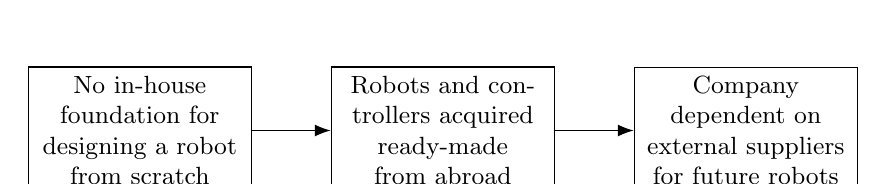
\begin{tikzpicture}[node distance=1cm, every node/.style={draw, rectangle, align=center, minimum height=1cm, text width=2.6cm, font=\small}, arrow/.style={-{Latex[length=2mm]}}]
\node (nofound) {No in-house foundation for designing a robot from scratch};
\node (import) [right=of nofound] {Robots and controllers acquired ready-made from abroad};
\node (dep) [right=of import] {Company dependent on external suppliers for future robots};
\draw[arrow] (nofound) -- (import);
\draw[arrow] (import) -- (dep);
\end{tikzpicture}
\caption{Status of in-house robot design capability before the project began.}
\label{fig:status_beginning}
\end{figure}

\subsection{Problem Definition}
\label{subsec:problem-definition}
\paragraph{Significance of the limitation:} The absence of any in-house foundation for designing robots, as described in Section~\ref{subsec:status-beginning}, is a limitation beyond simply relying on external suppliers. Without a design process of its own, the department has no way to create a new robot or control strategy tailored to its own needs — it can only work with whichever robots and controllers it already owns, all of which were imported ready-made from abroad.
\paragraph{Aim of project:} To begin addressing this gap, this project aims to design a quadruped robot and bring it into the Gazebo simulation environment, then develop a motion controller capable of producing basic locomotion gaits. Rather than solving the department's dependency on imports in full, the project is intended to establish a first, reusable example of an in-house robot design and development process that the department did not previously have.


\subsection{Related Literature}
\label{subsec:related-literature}

\paragraph{Inverse kinematics background:} The closed-form approach to inverse kinematics used in this project -- decomposing a leg's three-dimensional reach into a single ABAD angle followed by a two-link planar solve via the law of cosines -- follows a standard, well-established methodology in robotics rather than an ad hoc one. \citet{craig2017robotics} presents the same underlying two-link planar solution, including the same ambiguity between two candidate joint-angle solutions that is resolved in this project by selecting the smaller-magnitude angle (Section~\ref{sec:actuating-legs}, \Cref{app:ik-derivation}).

\paragraph{Leg odometry limitations:} Using leg kinematics together with a single IMU as the only proprioceptive sensing pathway, with no motion-capture system, GPS, or camera, is likewise an established approach in legged-robotics state estimation research rather than one specific to this project. \citet{bloesch2012state} show that under exactly this sensing configuration, roll, pitch, and body velocity are observable, but yaw and absolute position are not -- they can drift without bound unless an additional absolute reference, such as a magnetometer or a vision-based system, is introduced. This result directly motivates the scope and limitations discussed for the leg odometry estimator in Section~\ref{subsec:leg-odometry}.

\paragraph{Actuator choice rationale:} The decision to actuate each joint with a quasi-direct-drive actuator (Section~\ref{sec:modeling-export}) follows design principles developed for dynamic legged robots rather than being an arbitrary component choice. \citet{wensing2017proprioceptive} analyze proprioceptive actuator design in the MIT Cheetah, showing that low-gear-ratio, back-drivable actuation of this kind mitigates impact forces and enables high-bandwidth force control during locomotion -- the same actuation philosophy behind the CubeMars AK80-9 actuator used in this project's design.

\paragraph{Industry example:} Beyond academic research, platforms combining leg-based locomotion with onboard proprioceptive sensing and modular actuated joints are already deployed commercially. ANYbotics' ANYmal robot, for example, is sold and operated industrially for autonomous inspection tasks \citep{anybotics2026anymal}, showing that the overall architecture pursued in this project -- a legged robot relying on its own joint and inertial sensing rather than external infrastructure -- is a design direction already validated at commercial scale, and not merely an academic exercise.

\section{Internship Project}
\label{sec:internship-project}
\subsection{Project Objective}
\label{subsec:project-objective}
\paragraph{Project objective:} The objective of this project is to design a quadruped robot, or adapt a suitable existing model where one is available, and bring it into the Gazebo simulation environment in a physically accurate way. Once the robot has been properly modeled and imported, the second part of the objective is to develop a motion controller capable of producing basic locomotion gaits, starting with a statically stable crawl gait and, if time permits, extending to a dynamically stable gait such as trot.
\paragraph{Project scope:} The scope of the project centers on simulation: the primary deliverable is a working robot model and motion controller validated in Gazebo, not a physically assembled robot. However, the mechanical design itself targets physically realizable, off-the-shelf components, such as a specific commercially available actuator, so that a manufacturing path remains open even though building the robot is not a requirement of the project. Custom parts are not required to be entirely original where a suitable existing design can be sourced and adapted instead. Building and testing the resulting controller on physical hardware is a stretch goal to be attempted only if the simulation results are successful, and is not a required deliverable of the project itself.
\paragraph{Relation to the department's gap:} By producing this robot model and its motion controller, the project directly addresses the lack of an in-house design foundation described in Section~\ref{subsec:problem-definition}: rather than depending on ready-made imported robots, the department gains a reusable modeling and control-development pipeline that can be adapted to future robot designs.

\subsection{My Responsibilities}
\label{subsec:responsibilities}
\paragraph{My responsibilities:} This internship project was carried out entirely by myself, without a project partner. My contributions to the project can be listed as follows:

\begin{enumerate}
    \item \textbf{Mechanical Design:} I designed the quadruped robot's mechanical structure in CAD, including the body, legs, and joints, built around a specific actuator so that the resulting design could realistically be manufactured. For parts of this process, particularly detailed geometry and debugging, I made use of AI-assisted tools, directing and reviewing their output given my limited prior experience with CAD software.
    \item \textbf{Modeling and Export to Simulation:} I converted the CAD design into a simulation-ready model, computing the mass and inertia of each part from its geometry and exporting the complete robot to SDF format for use in Gazebo.
    \item \textbf{Inverse Kinematics:} I implemented the inverse kinematics needed to convert desired foot positions into joint angles for each leg.
    \item \textbf{Gait Planning and Motion Control:} I developed the motion controller responsible for planning and executing the robot's locomotion gaits, starting with a statically stable crawl gait.
    \item \textbf{Testing and Tuning:} I tested the robot and controller in simulation and tuned the controller's parameters based on the results.
    \item \textbf{Documentation and Reporting:} I documented the pipeline and methodology, and prepared this report along with a presentation summarizing the project.
\end{enumerate}

\subsection{Methodology/ Tools}
\label{subsec:methodology}
\paragraph{Tools and workflow:} Custom mechanical parts were designed parametrically in CadQuery, with AI assistance used for parts of the modeling process due to limited prior experience with CAD software. Where a suitable ready-made part, such as a leg design, was available online, it was sourced and adapted instead of being modeled from scratch. The resulting parts were reviewed manually in SolidWorks to check dimensions and fit, and SolidWorks was also used as part of the export process to SDF format. The physics and environment definitions were then edited directly in a text editor (Notepad++). The motion controller itself was written in Python using VS Code, and the whole system was simulated in Gazebo Sim (Windows-compatible version). For the motion controller, inverse kinematics was used to convert desired foot positions into joint angles for each leg, and a gait planning strategy was used to sequence leg movements into a coordinated locomotion pattern; both are described in detail in Section~\ref{subsec:details}.

\subsection{Expected Outcome and Deliverables}
\label{subsec:expected-outcome}
\paragraph{Success criteria and deliverables:} The project's objective is expected to be achieved through the closed-loop motion controller developed for the robot, which combines inverse kinematics, gait planning, and IMU-based stability feedback to keep the simulated robot balanced while executing a walking gait. The primary deliverable is a working control algorithm that allows the quadruped to walk stably, including on mildly unengineered terrain, with success defined as completing multiple full gait cycles without falling and achieving measurable net forward displacement. A secondary deliverable is the CAD model and .sdf files for the robot, whether custom-designed or adapted from sourced parts, structured so that they can be reused or adapted with only minor modification.

\subsection{Details}
\label{subsec:details}
\subsubsection{Modeling and Export to Gazebo Simulation Environment}
\label{sec:modeling-export}
\paragraph{Parametric design:} The quadruped robot was designed parametrically using CadQuery, a Python-based CAD tool, so that every dimension could be defined as a variable and the geometry regenerated as needed. The robot consists of a central body and four identical legs, each actuated by three joints: a hip abduction/adduction joint, a hip flexion joint, and a knee joint. The abduction/adduction joint gives each leg a lateral degree of freedom, which is needed to correct the robot's roll during walking, consistent with the leg architecture used in most real quadruped robots. The final assembled model is shown in \Cref{fig:quadruped_iso}.

\begin{figure}[htbp]
    \centering
    
\includegraphics[width=0.65\textwidth]{quadruped_manufacturable_isometric.png}
    \caption{Isometric view of the final quadruped assembly, rendered directly from the exported CAD model.}
    \label{fig:quadruped_iso}
\end{figure}

\paragraph{Actuator selection:} Each joint was actuated using a CubeMars AK80-9 quasi-direct-drive actuator, whose specifications are summarized in \Cref{tab:ak80_9_specs}, and the mechanical design was built around this specific, commercially available actuator so that the resulting model reflects a robot that could realistically be constructed. The design was intended to be mostly 3D-printed (PETG, nylon, and carbon-fiber-reinforced nylon), with a single CNC-machined aluminum bracket used only where load-bearing requirements exceeded what printed parts could handle. Since the actuator's exact mounting bolt pattern was not published by the manufacturer, all mounting interfaces were designed with slotted rather than fixed bolt holes to allow for adjustment once real hardware becomes available. The rationale for choosing this class of actuator is discussed further in Section~\ref{subsec:related-literature}.

\begin{table}[htbp]
    \centering
    \caption{CubeMars AK80-9 (KV100) actuator specifications.}
    \label{tab:ak80_9_specs}
    \begin{tabular}{ll}
        \hline
        Parameter & Value \\
        \hline
        Diameter & 98\,mm \\
        Thickness & 38.5\,mm \\
        Mass & 485\,g \\
        Rated (continuous) torque & 9\,Nm \\
        Peak torque & 18\,Nm \\
        Rated voltage & 48\,V \\
        \hline
    \end{tabular}
\end{table}

\paragraph{Hardest bracket geometry:} The bracket connecting the hip abduction/adduction actuator to the hip flexion actuator required particular care, since the two joints' rotation axes are perpendicular to one another; its geometry was derived analytically to route material around both actuators' cylindrical housings without intersecting either. All part positions and orientations were computed using an assembly system based on exact geometric relationships between parts, rather than positioned by eye. Since every joint in the design rotates about a single axis, a simplified pose-composition method was used to propagate each link's position and orientation from the body through each leg to the feet, rather than relying on a general-purpose three-dimensional rotation library.
\paragraph{Mass and inertia computation:} Mass and inertia values were computed directly from the CAD geometry rather than assumed: each actuator's mass was split between its stator and rotor sub-volumes, with the rotor's spin-axis inertia taken from the manufacturer's published specification and all other inertia values computed from the modeled geometry. For each link, the mass and inertia contributions of all physically co-located parts were combined using the parallel axis theorem to produce a single effective mass, center of mass, and inertia tensor. The resulting robot has a total mass of approximately 19\,kg, and each joint's torque limit in simulation was set to the actuator's 18\,Nm peak torque.
\paragraph{Final checks and export:} Once assembled, the complete model was checked for collisions between all parts, including between neighboring legs, to confirm that the geometry did not overlap anywhere. The final model was then exported to SDF format, together with the accompanying \texttt{model.config} metadata file required for Gazebo to recognize it as a valid model, and imported into the Gazebo simulation environment.

\subsubsection{Actuating the Legs with Basic Inverse Kinematics}
\label{sec:actuating-legs}
\paragraph{Two-step IK decomposition:} Each leg consists of three joints in series: an abduction/adduction joint (ABAD), a hip joint, and a knee joint, as shown in \Cref{fig:leg_geometry}. Because the ABAD joint's rotation axis is aligned with the body's forward axis, it can only move the leg within the plane perpendicular to that axis; the leg's forward/backward reach is determined entirely by the hip and knee. This structure allows the three-dimensional inverse kinematics problem to be decomposed into two simpler steps rather than solved as a single coupled system: first the ABAD angle is found as to align the hip-knee complex with the plane in which the desired foot location is at, and then the hip and knee angles are found from a standard two-link planar solve to bring the foot to the desired position on the pre-aligned plane.

\begin{figure}[htbp]
    \centering
    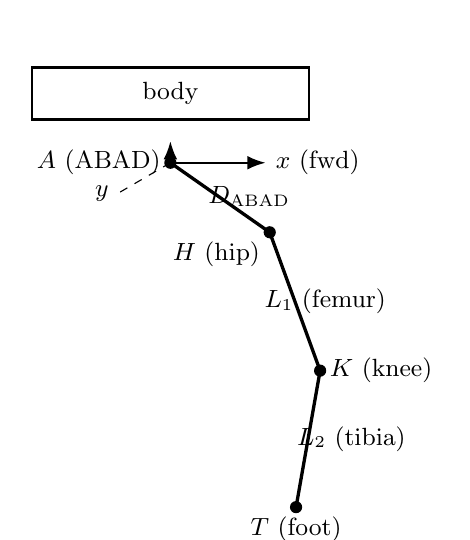
\begin{tikzpicture}[scale=1.1, every node/.style={font=\small}]
      % Body block
      \draw[thick] (-1.6,3.35) rectangle (1.6,3.95);
      \node at (0,3.65) {body};
      % ABAD joint
      \coordinate (A) at (0,2.85);
      \fill (A) circle (2pt);
      \node[left] at (A) {$A$ (ABAD)};
      \draw[-{Latex}, thick] (A) -- ++(1.1,0) node[right] {$x$ (fwd)};
      \draw[-{Latex}, thick] (A) -- ++(0,0.25);
      \draw[dashed] (A) -- ++(-0.6,-0.35) node[left] {$y$};
      % AH link
      \coordinate (H) at ($(A) + (-35:1.4)$);
      \draw[very thick] (A) -- (H);
      \fill (H) circle (2pt);
      \node[below left] at (H) {$H$ (hip)};
      \node at ($(A)!0.55!(H) + (0.28,0.05)$) {$D_{\text{ABAD}}$};
      % Femur
      \coordinate (K) at ($(H) + (-70:1.7)$);
      \draw[very thick] (H) -- (K);
      \fill (K) circle (2pt);
      \node[right] at (K) {$K$ (knee)};
      \node at ($(H)!0.5!(K) + (0.35,0)$) {$L_1$ (femur)};
      % Tibia
      \coordinate (F) at ($(K) + (-100:1.6)$);
      \draw[very thick] (K) -- (F);
      \fill (F) circle (2pt);
      \node[below] at (F) {$T$ (foot)};
      \node at ($(K)!0.5!(F) + (0.5,0)$) {$L_2$ (tibia)};
    \end{tikzpicture}
    \caption{Leg joint chain and link naming: ABAD joint $A$, which rotates around the robot's x axis, hip joint $H$, knee joint $K$, and foot $T$, which rotates around the axis aligned with the ABAD joint, connected by the fixed ABAD-to-hip offset $D_{\text{ABAD}}$, femur $L_1$, and tibia $L_2$.}
    \label{fig:leg_geometry}
\end{figure}

\paragraph{Solving the sub-problems:} The ABAD angle is found by treating the ABAD joint, hip joint, and target foot position as a right triangle in the plane perpendicular to the ABAD axis, since the hip and knee can only ever move the foot perpendicular to the ABAD-to-hip link; of the two candidate solutions this yields, the one smaller in magnitude is kept, and a solution exists only when the target lies outside a small unreachable region around the ABAD axis. Once the ABAD angle is known, the target is projected into the plane the hip and knee actually sweep through, which reduces the remaining problem to a standard two-link planar inverse kinematics solve (Section~\ref{subsec:related-literature}): the knee angle follows directly from the law of cosines, and the hip angle from decomposing the reach into components along and perpendicular to the femur, valid only when the target lies within the physical reach of the two links. The full closed-form expressions for all four joint angles are given in \Cref{app:ik-derivation}.
\paragraph{Closed-form implementation:} This closed-form solution was implemented directly in the leg controller rather than relying on an iterative or numerical solver, allowing each desired foot position to be converted into the corresponding joint angles in a single evaluation at every control cycle.

\subsubsection{Leg Odometry and State Feedback Estimation}
\label{subsec:leg-odometry}

\paragraph{Need for velocity and height estimates:} The gait planner does not simply replay a fixed foot trajectory: the stride length commanded to each leg is adjusted, tick by tick, based on the robot's own forward velocity, and the stance phase relies on knowing how far the body currently sits above the ground. Commanding these quantities open-loop -- that is, assuming the robot moves exactly as fast as it is told to -- would make the gait brittle to any disturbance, since the controller would have no way of detecting or correcting a mismatch between the commanded and actual motion. A closed-loop estimate of body velocity and height is therefore required. The simulated platform, however, exposes only two sources of proprioceptive information: the joint encoders on each leg, and the single body-mounted IMU described in Section~\ref{sec:modeling-export} (there is no external motion-capture system, GPS, or camera in the loop). \emph{Leg odometry} is the technique of recovering the missing velocity and height information from exactly these two sources, by treating a foot that is planted on the ground as a temporary, known reference point -- effectively using the leg itself as a position sensor.

\paragraph{Foot position from joint angles:} The forward kinematics problem is the inverse of the inverse-kinematics derivation of Section~\ref{sec:actuating-legs}: given the three measured joint angles of a leg, the same geometric parameters $L_1$, $L_2$, and $d_{\text{abad}}$ used there are applied in the opposite direction to compute the position of the foot relative to the body, $\mathbf{p}^{B}_{\text{foot}}(t) = (x_B, y_B, z_B)$. This vector is exact at every instant, since it depends only on the currently measured joint angles and the robot's fixed link geometry -- no integration or filtering is involved in computing it.

\paragraph{World-frame foot vector:} A body-frame foot position alone is not sufficient, because the body itself rotates during locomotion: pitch and roll change as load is transferred between stance legs, and yaw changes whenever the robot turns. To reason about where the foot actually is in the world, $\mathbf{p}^{B}_{\text{foot}}(t)$ must be re-expressed in world-frame coordinates using the body's current orientation. In this simulation, orientation is taken directly from the IMU sensor's orientation output (roll $\phi$, pitch $\theta$, and yaw $\psi$, derived from the quaternion described in Section~\ref{sec:modeling-export}), and used to build the rotation matrix $R(t) = R_z(\psi)\,R_y(\theta)\,R_x(\phi)$; the full expanded entries of $R(t)$ used in the implementation are given in \Cref{app:leg-odom-eqs} (Equation~\ref{eq:rotation-matrix}).

The world-frame foot vector is then $\mathbf{p}^{W}_{\text{foot}}(t) = \mathbf{p}^{W}_{\text{body}}(t) + R(t)\,\mathbf{p}^{B}_{\text{foot}}(t)$: the body-to-world rotation is what allows the two position vectors, expressed in two different, rotating bases, to be added together consistently.

\paragraph{Height without integration:} While a foot is in stance and in flat contact with the ground, its world-frame height does not change, by definition of contact. Taking the third (bottom) row of Equation~\eqref{eq:rotation-matrix} and inverting the height relationship above therefore gives the body's height directly from the current stance foot's body-frame coordinates and the current pitch and roll -- with no dependence on any past state and no time integration. It is also worth noting that the bottom row, $[-s_\theta,\ s_\phi c_\theta,\ c_\phi c_\theta]$, does not contain $\psi$ at all: the height estimate is exact regardless of any error in the yaw estimate, since a pure yaw rotation cannot change how far the body sits above a level floor.

\paragraph{Velocity by differentiation:} Horizontal velocity is obtained from the same relation. For a foot that remains planted, differentiating $\mathbf{p}^{W}_{\text{body}}(t) + R(t)\,\mathbf{p}^{B}_{\text{foot}}(t) = \text{const}$ with respect to time gives, by the product rule, two contributions: one from the leg's own joint angles changing, and one from the body itself rotating while the foot vector is held fixed. The full expansion is given in \Cref{app:leg-odom-eqs}. The leg-motion term is approximated by a finite difference of the body-frame foot position across one control tick, $\dot{\mathbf{p}}^{B}_{\text{foot}} \approx (\mathbf{p}^{B}_{\text{foot}}(t) - \mathbf{p}^{B}_{\text{foot}}(t-\Delta t))/\Delta t$; the body-rotation term is not dropped, but computed directly from the same IMU message's angular velocity reading and added in before the single rotation is applied, so the only remaining approximation is evaluating both terms once per tick rather than integrating exactly across it. This is the central reason leg odometry is used here instead of a double-integration of the IMU's accelerometer output: differentiating a bounded position quantity cannot accumulate the unbounded drift that comes from integrating a noisy acceleration signal once for velocity and twice for position, since there is no running sum of sensor error for the sensor noise to build up in.

\paragraph{Scope and limitations:} This estimator assumes that orientation itself is known, and in this simulation that assumption is met by reading the IMU's orientation output directly rather than reconstructing it from a realistic accelerometer--gyroscope--magnetometer fusion pipeline. This is a reasonable simplification for evaluating the gait and control design in simulation, but it should be stated explicitly as a limitation: a physical implementation would need to estimate orientation on board, and yaw in particular is a known hard case, with roll, pitch, and body velocity observable from leg kinematics and an IMU alone but yaw and absolute position not, as discussed in Section~\ref{subsec:related-literature}. The estimator described here inherits that same limitation in principle, even though it is masked in simulation by using the simulator's ground-truth orientation.

\subsubsection{Implemented Gaits and Gait Planning}
\label{sec:gaits}

\subsection{Results}
\label{subsec:results}



\section{Internship Experience}
\label{sec:internship-experience}
\subsection{Learning}
\label{subsec:learning}

\subsection{Relation to Undergraduate Education}
\label{subsec:relation-education}

\subsection{Difficulties}
\label{subsec:difficulties}

\subsection{A Typical Day}
\label{subsec:typical-day}

\section{Conclusions}
\label{sec:conclusions}

\section{Recommendations}
\label{sec:recommendations}

\newpage
\begingroup
\setstretch{1}
\setlength{\bibsep}{1em}   % adds the "blank line between references" spacing
\renewcommand{\bibsection}{\section*{\centering References}\addcontentsline{toc}{section}{References}}
\bibliographystyle{apalike}
\bibliography{references}
\endgroup

\newpage
\section{Appendices}
\label{sec:appendices}

\subsection{Full Inverse Kinematics Derivation}
\label{app:ik-derivation}
This appendix gives the complete derivation summarized in Section~\ref{sec:actuating-legs}. Given a desired foot position $(f_x, f_y, f_z)$ relative to the body, with sign flags $o_y$ and $s$ distinguishing the four mirrored legs, the ABAD angle is found by treating the ABAD joint, hip joint, and target as a right triangle in the plane perpendicular to the ABAD axis, since the hip and knee can only ever move the foot perpendicular to the ABAD-to-hip link. With target foot position expressed with respect to the ABAD joint, $d_y = o_y D_{\text{ABAD}} + f_y$ and $d_z = f_z$, this gives
\[
  r = \sqrt{d_y^2 + d_z^2}, \qquad
  c = \frac{o_y D_{\text{ABAD}}}{r}, \qquad
  \theta_{\text{abad}} = \operatorname{atan2}(d_z, d_y) \pm \arccos c .
\]
Of the two resulting candidate angles, the one smaller in magnitude is selected, since it corresponds to the hip remaining near its normal standing width rather than being pulled in toward the body's midline. A solution exists only when $r \ge D_{\text{ABAD}}$; targets closer to the ABAD axis than this fall inside a small unreachable region around the axis.

With $\theta_{\text{abad}}$ known, the target is projected into the plane the hip and knee actually sweep through by rotating $(d_y, d_z)$ by $-\theta_{\text{abad}}$:
\[
  w = -d_y \sin\theta_{\text{abad}} + d_z \cos\theta_{\text{abad}}, \qquad u = s\,f_x ,
\]
which reduces the remaining problem to a standard two-link planar inverse kinematics solve for the hip and knee, with target distance $r_2 = \sqrt{u^2+w^2}$.

The knee angle is found directly from the law of cosines, and the hip angle by decomposing the reach into components along and perpendicular to the femur:
\[
  \theta_{\text{knee}} = -\arccos\!\left(\frac{r_2^2 - L_1^2 - L_2^2}{2L_1L_2}\right), \qquad
  \theta_{\text{hip}} = \operatorname{atan2}(uk_1+k_2w,\; k_2u-k_1w),
\]
where $k_1 = L_1 + L_2\cos\theta_{\text{knee}}$ and $k_2 = L_2\sin\theta_{\text{knee}}$. This solution is only valid when $|L_1-L_2| \le r_2 \le L_1+L_2$, i.e. when the target lies within the physical reach of the two links.

\subsection{Leg Odometry: Rotation Matrix and Velocity Relation}
\label{app:leg-odom-eqs}
This appendix gives the full equations summarized in Section~\ref{subsec:leg-odometry}. Writing $c_\phi = \cos\phi$, $s_\phi = \sin\phi$ (and similarly for $\theta$, $\psi$) for compactness, the entries of the rotation matrix $R(t) = R_z(\psi)\,R_y(\theta)\,R_x(\phi)$ used in the implementation are

\begin{equation}
R(t) =
\begin{bmatrix}
c_\psi c_\theta & s_\phi s_\theta c_\psi - s_\psi c_\phi & s_\phi s_\psi + s_\theta c_\phi c_\psi \\
s_\psi c_\theta & s_\phi s_\psi s_\theta + c_\phi c_\psi & -s_\phi c_\psi + s_\psi s_\theta c_\phi \\
-s_\theta & s_\phi c_\theta & c_\phi c_\theta
\end{bmatrix}.
\label{eq:rotation-matrix}
\end{equation}

Differentiating the constraint $\mathbf{p}^{W}_{\text{body}}(t) + R(t)\,\mathbf{p}^{B}_{\text{foot}}(t) = \text{const}$, which holds while a foot remains planted, with respect to time gives, by the product rule,
\begin{equation}
\dot{\mathbf{p}}^{W}_{\text{body}}(t) = -\Big[\dot R(t)\,\mathbf{p}^{B}_{\text{foot}}(t) + R(t)\,\dot{\mathbf{p}}^{B}_{\text{foot}}(t)\Big].
\end{equation}
Using the rigid-body identity $\dot R(t) = R(t)\,[\boldsymbol\omega^{b}(t)]_\times$, where $\boldsymbol\omega^{b}(t)$ is the body-frame angular velocity read directly from the same IMU message that supplies orientation, the first term becomes $\dot R(t)\,\mathbf{p}^{B}_{\text{foot}}(t) = R(t)\big(\boldsymbol\omega^{b}(t) \times \mathbf{p}^{B}_{\text{foot}}(t)\big)$, a cross product computed entirely in body frame. Substituting gives the velocity relation actually used to obtain horizontal velocity by finite differencing:
\begin{equation}
\dot{\mathbf{p}}^{W}_{\text{body}}(t) \approx -R(t)\Big[\dot{\mathbf{p}}^{B}_{\text{foot}}(t) + \boldsymbol\omega^{b}(t) \times \mathbf{p}^{B}_{\text{foot}}(t)\Big].
\end{equation}

\end{document}
